\documentclass{article}
\usepackage{graphicx}
\usepackage{float}
\usepackage{amsmath}
\usepackage{amsfonts}
\usepackage{amssymb}
\usepackage{hyperref}
\usepackage{esint}
\usepackage[utf8]{inputenc}
\usepackage[a4paper, portrait, margin=0.75in]{geometry}
\setlength\parindent{0pt}
\usepackage[italian]{babel}
\usepackage{blindtext}

\usepackage{wasysym}


\hypersetup{
    colorlinks=true,
    linkcolor=black,
    filecolor=magenta,
    urlcolor=blue,
    pdftitle={APPLICAZIONI INDUSTRIALI ELETTRICHE ED ELETTRONICA},
    pdfpagemode=FullScreen,
}


\begin{document}
    \author{Ollari Ischimji Dmitri}
    \title{APPLICAZIONI INDUSTRIALI ELETTRICHE ED ELETTRONICA - lab?!}
    \date{Marzo 2022}

    \maketitle
    \tableofcontents

    \listoffigures
    \listoftables

    \section{Introduzione}

L'elettronica è la scienza e la tecnica inerente 
alla propagazione ed emissione degli elettroni nel vuoto o nella materia.

\subsection{Legge di Moore}
Il numero di transistori integrati nei chip raddopia ogni due anni.

\subsection{Trasduttore}
\begin{itemize}
    \item sensore: produce un segnale elettrico per una certa grandezza fisica
    \item attuatore: produce una certa grandezza fisica per un segnale elettrico
\end{itemize}

\subsection{Segnale}
Funzione del tempo che rappresenta la variazione di una grandezza fisica.

\subsubsection{I segnali elettrici}
Possono essere analogici(livelli continui nel tempo) o digitali(livelli discreti).

\subsection{Circuiti digitali}
\begin{figure}[H]
    \centering
    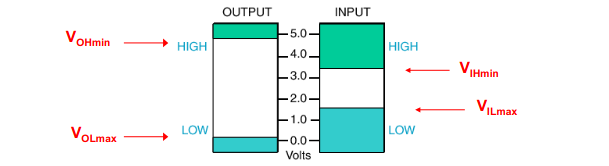
\includegraphics[width=0.5\linewidth]{imgs/0 - livelli-input-output}
    \caption{Livelli input output}
    \label{fig:input_output_livelli}
\end{figure}

\begin{itemize}
    \item $V_{OHmin}$ è la minima tensione in output corrispondente ad un 1 logico
    \item $V_{OLmax}$ è la massima tensione in output corrispondente ad un 0 logico
    \item $V_{IHmin}$ è la minima tensione per avere un 1 logico
    \item $V_{ILmax}$ è la massima tensione per avere un 0 logico
    \item I margini di rumore sono $V_{OHmin} - V_{IHmin}$
    \item I margini di rumore sono $V_{ILmax} - V_{OLmax}$
\end{itemize}

\subsection{Digitale vs Analogico}
\begin{itemize}
    \item elevata potenzialità di calcolo ed elaborazioni del segnale
    \item maggior robustezza a disturbi e rumore
    \item minor sensibilità alle variazioni di temperatura ed alle tolleranze dei parametri del dispositivo
\end{itemize}

\subsection{Analogico vs Digitale}
\begin{itemize}
    \item in natura le grandezze sono continue(segnali analogici)
    \item sensori: grandezza fisica -> ingresso analogico
    \item attuatori: segnale -> uscita analogica
    \item si usano circcuiti di conversione A/D e D/A
\end{itemize}
\subsubsection{ADC}
Converte un input analogico ad un output digitale, si fa una approssimazione dell'input con il
campionamento.

\subsubsection{DAC}
Converte digitale verso analogico.

    \section{Semiconduttori}
\subsection{Classificazione dei materiali}
Ressitività $\rho$:
\begin{itemize}
    \item $\rho < 10^{-1}\Omega\cdot cm$ è un conduttore
    \item $10^{-1}\Omega\cdot cm < \rho < 10^{5}\Omega\cdot cm $ è un semiconduttore
    \item $10^{5}\Omega\cdot cm < \rho$ è un isolante
\end{itemize}

\subsubsection{Caratteristiche dei semiconduttori}
\begin{itemize}
    \item resistività intermedia tra isolanti e conduttori
    \item possibilità di variare $\rho$ mediante il drogaggio
    \item due portatori di carica liberi: elettrone(-) e lacuna(+)
    \item disponibili sia come cristalli che come composti
\end{itemize}

\subsubsection{Silicio: legame covalente}
4 elettroni poco legati(di valenza)
\begin{itemize}
    \item non sono legati strettamente al nucleo
    \item risentono dell'interazione deglie altri atomi
    \item formano un doppio legame covalente con gli altri atomi
\end{itemize}

\subsection{Drogaggio di un semiconduttore}

Il drogaggio è l'aggiunta di atomi diversi, esistono 2 tipi di drogaggio:
\begin{itemize}
    \item drogaggio di tipo n: aggiunta di elementi del quinto gruppo(As,P,Sb)
    \item drogaggio di tipo p: aggiunta di elementi del terzo gruppo(B)
\end{itemize}


\subsubsection{Silicio di tipo n}
Vengono aggiunti al silicio elementi del quinto gruppo, il quinto elettrone di valenza si lega debolmente al nucle
e non è impiegato in legami covalenti.
L'elettrone può facilmente liberarisi dal nucleo per effetto dell'energia termica.


Il quinto elettrone può muoversi nel cristallo.

\subsubsection{Silicio di tipo p}
Essendo il drogaggio effettuato con un elemento del terzo gruppo, manca un elettrone nel legame
covalente(\textbf{lacuna}).

È facile catturare un elettrone per questa configurazione.

La cattura di un elettrone da parte di questa configurazione, crea una lacuna in una molecola vicina,
viene creata una rezione a catena dove questa lacuna si "sposta" all'interno degli atomi adiacenti.

Si parla di "moto di lacune" anche se sono comunque gli elettroni a muoversi.

\subsection{Corrente di "drift"}
\begin{figure}[H]
    \centering
    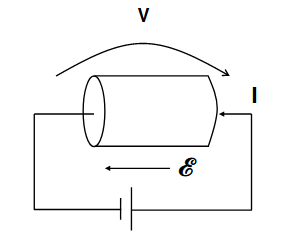
\includegraphics[width=0.3\linewidth]{imgs/corrente-di-drift}
    \caption{Corrente di drift}
    \label{fig:corrente_drift}
\end{figure}
Forza di trascinamento sull'elettrone
\begin{equation*}
    F = -q \epsilon
\end{equation*}

Forza di trascinamento sulla lacuna
\begin{equation*}
    F = q \epsilon
\end{equation*}

Per campi elettrici moderati esiste una relazione lineare fra intensità del campo
$\epsilon$ e \textbf{velocità del portatore di carica}.

Materiali ad alta mobilità($\mu$) hanno una velocità media dei portatori molto alta.


\begin{figure}[H]
    \centering
    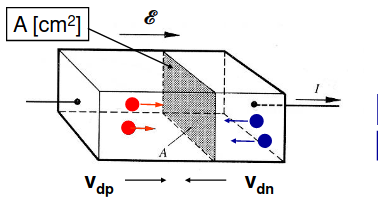
\includegraphics[width=0.3\linewidth]{imgs/corrente}
    \caption{Corrente}
    \label{fig:corrente}
\end{figure}

Dove le forse sono:
\begin{itemize}
    \item
        \begin{equation*}
            I_n = -qn(-V_{dn})A = qnV_{dn}A
        \end{equation*}
    \item
        \begin{equation*}
            I_p = qpV_{dp}A
        \end{equation*}
\end{itemize}

La $A$ sta per la superficie attraversata perchè la corrente è il numero di lacune che attraversano la superficie in un 
tempo.

La densità si ottiene dividendo per l'Area.

La J rappresenta la densità di corrente:
\begin{equation*}
    J = J_p + J_n = q(p_\mu_p + n\mu_n)\cdot \epsilon
\end{equation*}
Da cui si ottiene la legge di \textbf{ohm locale}:
\begin{equation*}
    J = \sigma \cdot \epsilon
\end{equation*}

Dove la $\sigma$ rappresenta la conducibilità:
\begin{equation}
    \sigma = \frac{1}{\rho} = q(p_\mu_p + n\mu_n)
\end{equation}
dove $\rho$ rappresenta la resistività.

\subsubsection{Drift: metalli vs semiconduttori}
Nei metalli e nei semiconduttori, il drift è simile, tranne per il fatto che nei metalli non vi sono lacune come
portatori di carica.
E ovviamente che la conducibilità di un metallo è molto maggiroe di quella di un semiconduttore.

\subsection{Diffusione}
Meccanismo di trasporto rilevante solo nei semiconduttori, simile alal diffusione dei gas causata da una
differenza di concetrazione dei portatori.

\subsubsection{Diffusione: elettroni}
 \begin{equation}
     J_n=-(-q)D_n\frac{dn}{dx} = qD_n\frac{dn}{dx}
 \end{equation}
essendo l'elettrone negativo si prende la crica q con carica negativa, il segno meno iniziale rappresenta
il flusso verso la zona a minor intensità.

\subsubsection{Diffizione: lacune}
\begin{equation}
    J_p=-qD_p\frac{dp}{dx}
\end{equation}


\subsection{Legge del trasporto "drift-diffusione"}

I due meccanismi di trasporto per le due cariche sono:
elettrone:
\begin{equation}
    J_n= qn\mu_n\epsilon + qD_n\frac{dn}{dx}
\end{equation}
lacuna:
\begin{equation}
    J_p= qp\mu_p\epsilon - qD_p\frac{dp}{dx}
\end{equation}

Il \textbf{DRIFT} tipicamente è dominante per i \textbf{maggioritari}: $J_{n-drift} \propto n\epsilon$.


La \textbf{DIFFUSIONE} tipicamente è dominante per i \textbf{minoritari}: $J_{n-diff} \propto \frac{dn}{dx}$.


    \section{Diodo a giunzione}
\subsection{Giunzione p-n}

Si ottiene al contatto tra due regioni di un semiconduttore, uno drogato con p e uno con n.
\subsubsection{FOrmazione della giunzione}
Il diodo è formato da due parti, anodo(A) semiconduttore drogato del tipo P e catodo(K) semiconduttore del tipo N.

Nel diodo si instaura un campo elettrico $\sigma$ che ostacola il fluire delle cariche(rende la corrente nulla).

\begin{figure}[H]
    \centering
    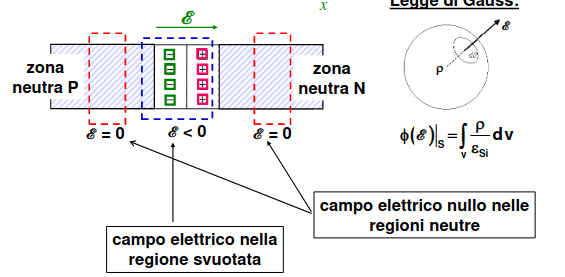
\includegraphics[width=0.5\linewidth]{imgs/giunzione-svuotata}
    \caption{Rappresentazioni regione svuotata e zona neutra}
    \label{fig:reg_svuot_neutr}
\end{figure}

\subsubsection{Regione svuotata: potenziale V}
\begin{equation}
    \epsilon = -\frac{dV}{dx}
\end{equation}
Si crea una caduta di potenziale agli estremi della regione svuotata.
Se si prende come 0 l'anodo(P) si ottiene un risultato positivo di tensione $V=V_{bi}$(potenziale di built-in).

\begin{figure}[H]
    \centering
    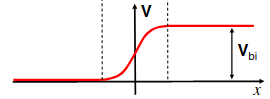
\includegraphics[width=0.4\linewidth]{/home/dmo/git/appunti-latex-2021-2022/APPLICAZIONI INDUSTRIALI ELETTRICHE ED ELETTRONICA/imgs/tensione-built-in}
    \caption{Tensione built-in}
    \label{fig:built-in}
\end{figure}


\subsection{Diodo polarizzato in diretta ($V_D>0$)}
\begin{figure}[H]
    \centering
    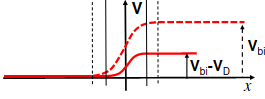
\includegraphics[width=0.4\linewidth]{imgs/polarizzato-direttamente}
    \caption{Diodo polarizzato direttamente}
    \label{fig:polarizzato-direttamente}
\end{figure}

Si abbassa la barriera che inpediva il fluire della corrente.
\subsubsection{Caratteristiche $I_D(V_D)$ in diretta}
\begin{equation}
    I_D = I_S(e^{\frac{V_D}{V_T} - 1}) \cong I_{S}e^{\frac{V_D}{V_T}}
\end{equation}

Dove la tensione del diodo della tensione termica($V_D >> V_T$).

Tensione termica:
\begin{equation*}
    V_T = \frac{kT}{q}
\end{equation*}
La tensione termica con temperatura $300K$ è $25,6mV$.

La $I_S$ è la corrente inversa di saturazione.

La tensione del diodo si approssima a circa $V_D = \cong 0,7V$

\subsection{Diodo polarizzato in inversa e breakdown ($V_D < 0$)}

Essendo una tensione negativa, la "barriera" che inpediva il fluire della corrente viene aumentata.

\subsubsection{Breakdown a valanga}
Il diodo il polarizzazione inversa, regge la tensione fin al punto di breakdown senza far passare la corrente,
dopodichè cede, distruggendosi.

\begin{figure}[H]
    \centering
    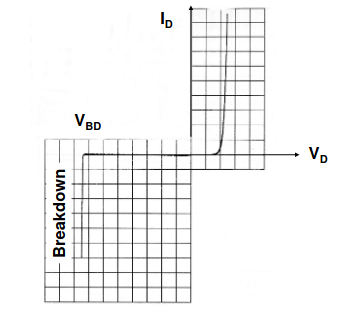
\includegraphics[width=0.3\linewidth]{imgs/breakdown}
    \caption{comportamento reale del diodo}
    \label{fig:breakdown}
\end{figure}

\subsection{Applicazione del diodo}
\subsubsection{Raddrizzatore}
\begin{figure}[H]
    \centering
    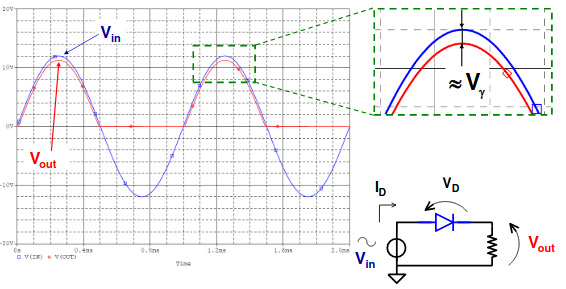
\includegraphics[width=0.7\linewidth]{imgs/radrizzatore}
    \caption{radrizzatore}
    \label{fig:radrizzatore}

\end{figure}
Solitamente si utilizzano i diodi zener che hanno una tensione di breakdown enorme se si vogliono usare come
radrizzatori di un segnale alternato.

\subsubsection{Rilevatori di picco}
\begin{figure}[H]
    \centering
    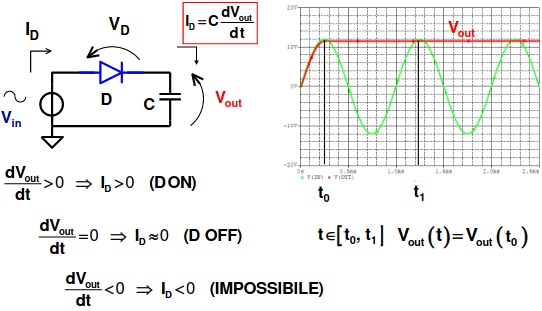
\includegraphics[width=0.8\linewidth]{imgs/rilevatore-di-picco}
    \caption{rilevatore di picco}
    \label{fig:rilevatore-di-picco}
\end{figure}

\subsection{Capacità del diodo e modello circuitale}
La capacità per la tensione del diodo($0.7V$):
\begin{equation}
    Q_J(V_D) = K_j \sqrt {V_{bi} - V_D}
\end{equation}

\begin{figure}[H]
    \centering
    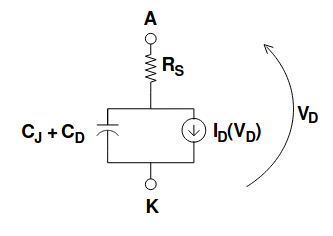
\includegraphics[width=0.5\linewidth]{imgs/modello-del-diodo}
    \caption{modello del diodo}
    \label{fig:modello-del-diodo}
\end{figure}




















\end{document}